
\section{Scanning strategy}
\label{se:scan_strat}

\begin{itemize}
\item explain how the 4f harmonics separates from the scanning frequencies
\item derive constraints on precession, nutation and scanning speed vs HWP
  speed.
\item Number of samples per beam vs combination of kids to produce a map: one
  map is the average of N independent maps *only* if *each* KID produces a full
  map. Otherwise it's a somehow classic combination of different detectors
\end{itemize}

A key factor in the design of space experiments is the scanning strategy of the instrument, as it conditions all the observations. Here, we present different simulations of scanning strategies such as the ones used in EPIC \citep{2009arXiv0906.1188B}, and Planck \citep{2005A&A...430..363D}. \\

Fig.~\ref{fig:satellite} shows a representation of a satellite, where $\alpha$ is the angle between the spin axis and the precession axis, and $\beta$ is the angle between the optical and spin axis of the satellite.
For EPIC scanning strategy, the optical axis of the telescope is inclined by $\beta$=55$\degree$ with respect to the spin axis The spin axis is inclined by $\alpha$=45$\degree$ from the precession axis and it precesses around the Sun-Earth axis every hour.
Planck scans large circles on the sky with a 85$\degree$ angle between the optical axis and the spin axis. The precession angle is 7$\degree$.

\begin{figure}[h]
  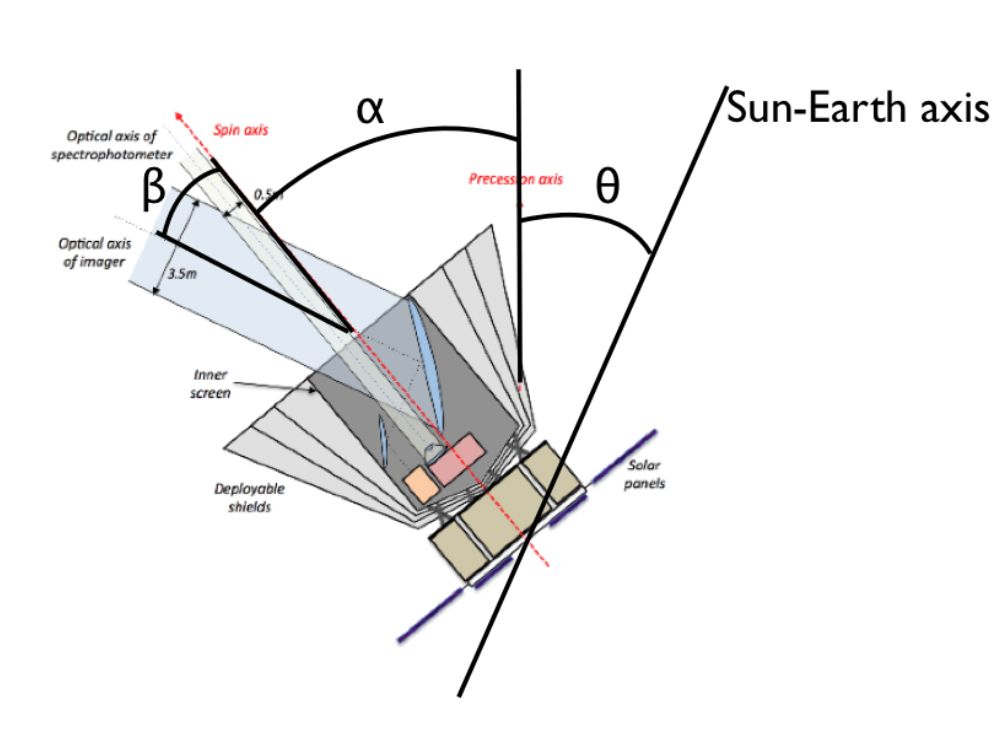
\includegraphics[clip,angle=0,width=\columnwidth]{Figures/schema_satellite.png}
  \caption{Schematic view of a satellite}
  \label{fig:satellite}
\end{figure}

The two scanning strategies are represented in Fig.~\ref{fig:strat-polsat-Planck}.

\begin{figure}[h]
  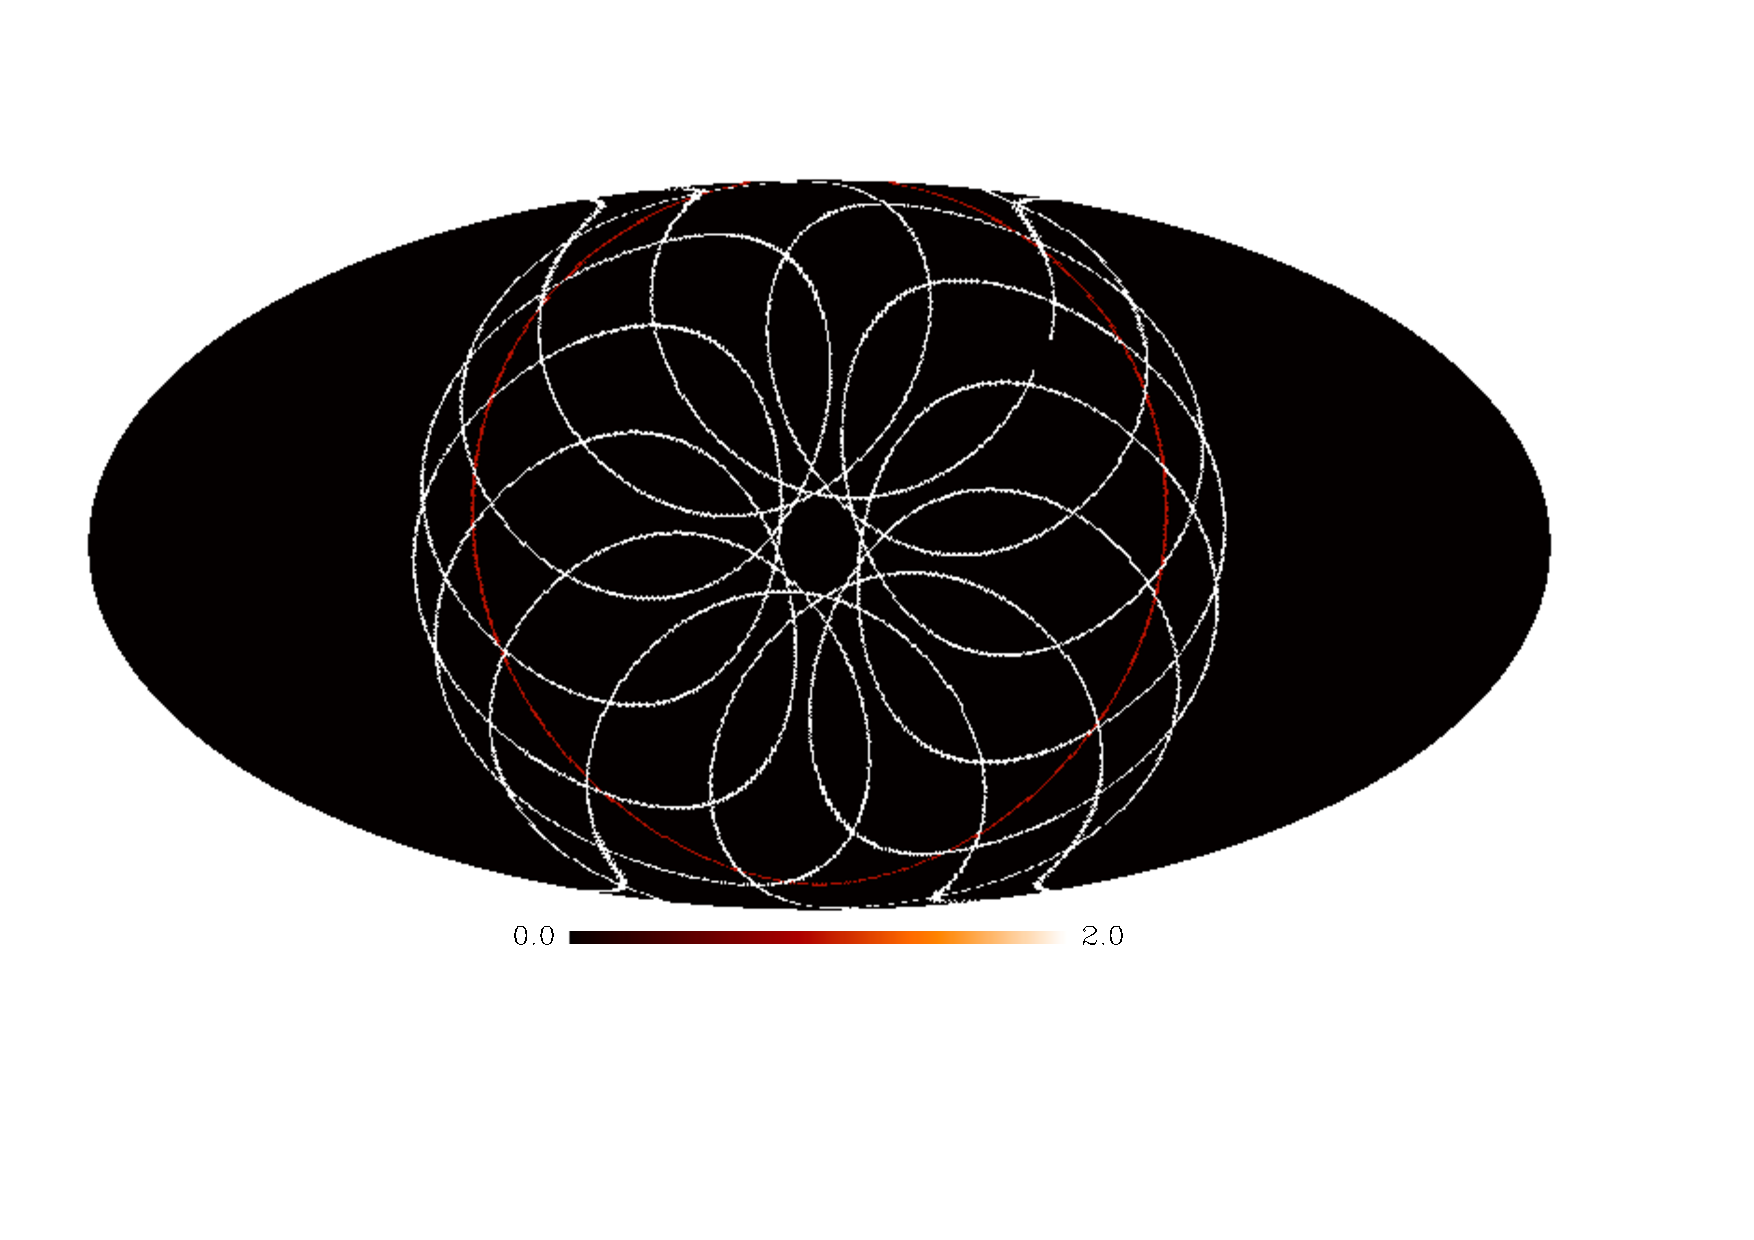
\includegraphics[clip,angle=0,width=\columnwidth]{Figures/plot_mollweide.pdf}
  \caption{White : representation of EPIC scanning strategy. Red : representation of Planck scanning strategy }
  \label{fig:strat-polsat-Planck}
\end{figure}

In the context of a CMB experiment mapping a large fraction of the sky, one should also consider the CMB dipole  with its 6.73\,mK peak to peak \citep{2015IJMPD..2430004B} converts into a \todo{XXX\,Jy} signal. The CMB dipole is a smooth gradient in the CMB temperature accross the sky. It is the result of the motion of the local group of galaxies with respect to the reference framed defined by the CMB. The CMB dipole amplitude is $\Delta T = 3.365 \pm 0.027$ mK and directed toward $(l,b) = (264.4 \degree \pm 0.3 \degree , 48.4 \degree \pm 0.5 \degree)$ in galactic coordinates \citep{1993ApJ...419....1K}. It can displace the zero level $Z$ along the circle so that a bright source would enter the non linear regime sooner than expected. This is also true for strong Galactic emission like that of Dust at frequencies above $\sim 100$\,GHz. 

\begin{figure}[h]
  \includegraphics[clip,angle=0,width=\columnwidth]{Figures/histo_galaxy_dipole_planck.eps}
  \caption{Histogram of flux of Galaxy with Planck scanning strategy}
  \label{fig:histo_galaxy_dipole}
\end{figure}

%Here we scan a map of the Galaxy with the two pointing strategies described earlier. In addition to the Galaxy, there is another signal that we have to take into account which is the CMB dipole. The CMB dipole is a smooth gradient in the CMB temperature accross the sky. It is the result of the motion of the local group of galaxies with respect to the reference framed defined by the CMB. The CMB dipole amplitude is $\Delta T = 3.365 \pm 0.027$ mK and directed toward $(l,b) = (264.4 \degree \pm 0.3 \degree , 48.4 \degree \pm 0.5 \degree)$ in galactic coordinates \citep{2015IJMPD..2430004B}. Like in the precedent simulations we add the template of HWP that we subtract after the signal goes through the KID model.
%
%We have seen previously that to be in a linear regime, constraints had to be put on the scanning strategy, especially on the scanning speed, and on the incoming flux. Here the scanning strategy that we use ensure that we respect the Nyquist criteria, by having a number of points per beam between 3 and 5. Plus, we can see in Fig.~\ref{fig:histo-gal-dip}, that the flux of the Galaxy and Dipole does not go higher than 20 Jy and that the two methods \rf\ and \cf\ can reconstruct it.


%% \todo{keep for global conclusion:} In conclusion, because we can not directly
%% measure the optical power from a KID, new methods were developed to monitor the
%% shift of the resononance frequency of the detector. First with the modulated
%% readout technique we can calculate four quantities : $\I$, $\Q$, $\di$,
%% $\dq$. With these quantities in hand, we can monitor the shift of the resonant
%% frequency and derive the corresponding incident power ny using the two methods
%% that were developed : \rf\ which is already successfully used in \nika\ and
%% \nika2\ (see \citep{2014A&A...569A...9C}) , and \cf\ which is an improvement
%% from \rf . In this paper, we compare these two methods in terms of linearity. To
%% do so, in the next sections we do simulations of observations by a KID and we
%% use \rf\ and \cf\ to reconstruct the signal. We then study the impact of the KID
%% non-linearity on the search for B modes polarization of the CMB.

